% !TEX TS-program = xelatex
% !TEX encoding = UTF-8
\documentclass{article}

\usepackage{amsmath,amssymb,amsfonts}
\usepackage{graphicx}
\usepackage{xcolor}
\usepackage{geometry}
\geometry{top = 1.5 cm, bottom = 1.5 cm}


\title{Revisit to the theoretical analysis of a classical piezoelectric cantilever energy harvester}
\author{Maoying Zhou}
\date{\today}

\begin{document}

\maketitle

\section{Summary of the interested equations}

The dynamic equations for a typical piezoelectric composite cantilever beam is 
\begin{equation}
    B_p \frac{\partial^4 w(x,t)}{\partial x^4} + m_p \frac{\partial^2 w(x,t)}{\partial t^2} = 0,
\end{equation}
where $B_p$ is the equivalent bending stiffness and $m_p$ is the line mass density of the piezoelectric cantilever beam. If the piezoelectric elements attached to the cantilever beam is connected to an external electrical load $R_l$, we have 
\begin{equation}
    \frac{d Q_p(t)}{d t} + \frac{V_p(t)}{R_l} = 0.
\end{equation}
For the underlying physics, we have the following constitutive equations
\begin{equation}
    \begin{aligned}
        M_p(x,t) &= B_p \frac{\partial^2 w(x,t)}{\partial x^2} - e_p V_p(t), \\
        q_p(x,t) &= e_p \frac{\partial^2 w(x,t)}{\partial x^2} + \varepsilon_p V_p(t),
    \end{aligned}
\end{equation}
or equivalently,
\begin{equation}
    \left\{\begin{aligned}
        M_p(x,t) &= B_p \frac{\partial^2 w(x,t)}{\partial x^2} - e_p V_p(t), \\
        Q_p(x,t) &= e_p \left.\left[ \frac{\partial w(x,t)}{\partial x} \right]\right|_0^{l_p} + C_p V_p(t).
    \end{aligned}\right.
\end{equation}

One end of the cantilever beam is fixed while the other end is free. So the boundary conditions are
\begin{equation}
    \left\{\begin{aligned}
        w(0,t) &= w_b(t), \\
        \frac{\partial w(0,t)}{\partial x} &= 0,
    \end{aligned}\right.
\end{equation}
and
\begin{equation}
    \left\{\begin{aligned}
        M_p(l_p,t) &= B_p \frac{\partial^2 w(l_p,t)}{\partial x^2} - e_p V_p(t) = 0, \\
        N_p(l_p,t) &= \frac{\partial M_p(l_p,t)}{\partial x} = B_p \frac{\partial^3 w(l_p,t)}{\partial x^3} = 0.
    \end{aligned}\right.
\end{equation}


In the classical energy harvesting applications, the cantilever beam is subject to a periodical base excitation $w_b(t)$. Thus the dynamic response of the cantilever beam is decomposed as 
\begin{equation}
    w(x,t) = w_b(t) + w_{rel}(x,t),
\end{equation}
where $w_{rel}(x,t)$ is the relative displacement function of the cantilever beam. In this way, the system is converted into 
\begin{equation}
    B_p \frac{\partial^4 w_{rel}(x,t)}{\partial x^4} + m_p \frac{\partial^2 w_{rel}(x,t)}{\partial t^2} = - m_p \frac{\partial^2 w_{b}(t)}{\partial t^2},
\end{equation}
\begin{equation}
    e_p \left.\left[ \frac{\partial^2 w_{rel}(x,t)}{\partial x \partial t}\right]\right|_0^{l_p} + C_p \frac{d V_p(t)}{d t} + \frac{V_p(t)}{R_l} = 0.
\end{equation}
\begin{equation}
    \left\{\begin{aligned}
        w_{rel}(0,t) &= 0, \\
        \frac{\partial w_{rel}(0,t)}{\partial x} &= 0,
    \end{aligned}\right.
\end{equation}
and
\begin{equation}
    \left\{\begin{aligned}
        B_p \frac{\partial^2 w_{rel}(l_p,t)}{\partial x^2} - e_p V_p(t) &= 0, \\
        \frac{\partial^3 w_{rel}(l_p,t)}{\partial x^3} &= 0.
    \end{aligned}\right.
\end{equation}

Considering a sinusoidal base excitation
\begin{equation}
    w_b(t) = \eta_b e^{j \sigma_b t}
\end{equation}
where $\xi_b$ is usually a real vibration amplitude, the steady state solution for the above system can be reasonably set as
\begin{equation}
    w_{rel}(x,t) = \eta_{rel}(x) e^{j \sigma_b t},\quad V_p(t) = \tilde{V}_p e^{j \sigma_b t},
\end{equation}
where $\eta_{rel}(x)$ and $\tilde{V}_p$ are complex amplitudes. Then the above system is again simplified as 
\begin{equation}
    B_p \frac{\partial^4 \eta_{rel}(x)}{\partial x^4} - m_p \sigma_b^2 \eta_{rel}(x) = m_p \sigma_b^2 \eta_{b},
\end{equation}
\begin{equation}
    \left\{\begin{aligned}
        \eta_{rel}(0) &= 0, \\
        \frac{\partial \eta_{rel}(0)}{\partial x} &= 0,
    \end{aligned}\right.
\end{equation}
and
\begin{equation}
    \left\{\begin{aligned}
        B_p \frac{\partial^2 \eta_{rel}(l_p)}{\partial x^2} + \frac{j \sigma_b R_l }{1 + j \sigma_b C_p R_l } e_p^2 \frac{\partial \eta_{rel}(l_p)}{\partial x} &= 0, \\
        \frac{\partial^3 \eta_{rel}(l_p)}{\partial x^3} &= 0.
    \end{aligned}\right.
\end{equation}
\textcolor{red}{Note that here we assume a sinusoidal steady state response, which is not actually validated theoretically. }


Obviously we can have the following dimensionless scheme:
\begin{equation}
    \eta_{rel} \sim u \eta_b ,\quad x \sim z l_p 
\end{equation}
and therefore the following dimensionless parameters
\begin{equation}
    \sigma = \sigma_b \sqrt{\frac{m_p l_p^4}{B_p}}, \quad \beta = R_l C_p \sqrt{\frac{B_p}{m_p l_p^4}}, \quad \delta = \frac{e_p^2 l_p}{C_p B_p}.
\end{equation}
Now, we reach the following dimensionless system of boundary value problem
\begin{equation}
    \left\{\begin{aligned}
        u^{\prime\prime\prime\prime} -\sigma^2 u &= \sigma^2, \\
        u(0) &= 0, \\
        u^{\prime}(0) &= 0, \\
        u^{\prime\prime}(1)  + \frac{j \beta \sigma }{1 + j \beta \sigma } \delta u^{\prime}(1) &= 0, \\
        u^{\prime\prime\prime}(1) &= 0,
    \end{aligned}\right.
\end{equation}
where the prime denotes the derivative with respect to $z$. The analytical solution to this problem can be formulated as
\begin{equation}
    u(z;\delta) = A_\delta \cos{\sqrt{\sigma}z} + B_\delta \sin{\sqrt{\sigma}z} + C_\delta \cosh{\sqrt{\sigma}z} + D_\delta \sinh{\sqrt{\sigma}z} - 1
    \label{eq:eq_disp_func_general_coeffs}
\end{equation}
and hence
\begin{equation}
    \begin{aligned}
        u^{\prime}(z;\delta) &= \sigma^{1/2} \left( - A_\delta \sin{\sqrt{\sigma}z} + B_\delta \cos{\sqrt{\sigma}z} + C_\delta \sinh{\sqrt{\sigma}z} + D_\delta \cosh{\sqrt{\sigma}z} \right), \\
        u^{\prime\prime}(z;\delta) &= \sigma  \left( - A_\delta \cos{\sqrt{\sigma}z} - B_\delta \sin{\sqrt{\sigma}z} + C_\delta \cosh{\sqrt{\sigma}z} + D_\delta \sinh{\sqrt{\sigma}z} \right), \\
        u^{\prime\prime\prime}(z;\delta) &= \sigma^{3/2} \left( A_\delta \sin{\sqrt{\sigma}z} - B_\delta \cos{\sqrt{\sigma}z} + C_\delta \sinh{\sqrt{\sigma}z} + D_\delta \cosh{\sqrt{\sigma}z} \right). 
    \end{aligned}
\end{equation}
The coefficients $A_\delta$, $B_\delta$, $C_\delta$, and $D_\delta$ are then subject to the following linear system of equations:
\begin{equation}
    \left\{\begin{aligned}
        A_\delta + C_\delta &= 1, \\
        B_\delta + D_\delta &= 0, \\
        \left( - A_\delta \cos{\sqrt{\sigma}} - B_\delta \sin{\sqrt{\sigma}} + C_\delta \cosh{\sqrt{\sigma}} + D_\delta \sinh{\sqrt{\sigma}} \right) &+ \\
        \frac{j \beta \sqrt{\sigma}}{ j\sigma \beta + 1 } \delta \left( - A_\delta \sin{\sqrt{\sigma}} + B_\delta \cos{\sqrt{\sigma}} + C_\delta \sinh{\sqrt{\sigma}} + D_\delta \cosh{\sqrt{\sigma}} \right) &= 0, \\
        A_\delta \sin{\sqrt{\sigma}} - B_\delta \cos{\sqrt{\sigma}} + C_\delta \sinh{\sqrt{\sigma}} + D_\delta \cosh{\sqrt{\sigma}} &= 0.
    \end{aligned}\right.
\end{equation}


Analytically, we can directly obtain the solution to this problem as 
\begin{equation}
    \left\{\begin{aligned}
        A_\delta &= \frac{ 1 + \cos\sqrt{\sigma } \cosh\sqrt{\sigma } - \sin\sqrt{\sigma } \sinh\sqrt{\sigma} + \frac{2 j \beta \sqrt{\sigma}}{ 1+ j \beta \sigma } \delta \left( \cos\sqrt{\sigma } \sinh\sqrt{\sigma } \right)}{2 \left[ 1 + \cos\sqrt{\sigma } \cosh\sqrt{\sigma } + \frac{j \beta \sqrt{\sigma}}{ 1+ j \beta \sigma } \delta \left( \cos\sqrt{\sigma } \sinh\sqrt{\sigma } + \sin\sqrt{\sigma } \cosh\sqrt{\sigma } \right) \right]}, \\
        B_\delta &= \frac{ \cos\sqrt{\sigma } \sinh\sqrt{\sigma } + \sin\sqrt{\sigma } \cosh\sqrt{\sigma} + \frac{2 j \beta \sqrt{\sigma}}{ 1+ j \beta \sigma } \delta \left( \sin\sqrt{\sigma } \sinh\sqrt{\sigma } \right)}{2 \left[ 1 + \cos\sqrt{\sigma } \cosh\sqrt{\sigma } + \frac{j \beta \sqrt{\sigma}}{ 1+ j \beta \sigma } \delta \left( \cos\sqrt{\sigma } \sinh\sqrt{\sigma } + \sin\sqrt{\sigma } \cosh\sqrt{\sigma } \right) \right]}, \\
        C_\delta &= \frac{ 1 + \cos\sqrt{\sigma } \cosh\sqrt{\sigma } + \sin\sqrt{\sigma } \sinh\sqrt{\sigma} + \frac{2 j \beta \sqrt{\sigma}}{ 1+ j \beta \sigma } \delta \left( \sin\sqrt{\sigma } \cosh\sqrt{\sigma } \right)}{2 \left[ 1 + \cos\sqrt{\sigma } \cosh\sqrt{\sigma } + \frac{j \beta \sqrt{\sigma}}{ 1+ j \beta \sigma } \delta \left( \cos\sqrt{\sigma } \sinh\sqrt{\sigma } + \sin\sqrt{\sigma } \cosh\sqrt{\sigma } \right) \right]}, \\
        D_\delta &= \frac{ -\cos\sqrt{\sigma } \sinh\sqrt{\sigma } - \sin\sqrt{\sigma } \cosh\sqrt{\sigma} -  \frac{2 j \beta \sqrt{\sigma}}{ 1+ j \beta \sigma } \delta \left( \sin\sqrt{\sigma } \sinh\sqrt{\sigma } \right)}{2 \left[ 1 + \cos\sqrt{\sigma } \cosh\sqrt{\sigma } + \frac{j \beta \sqrt{\sigma}}{ 1+ j \beta \sigma } \delta \left( \cos\sqrt{\sigma } \sinh\sqrt{\sigma } + \sin\sqrt{\sigma } \cosh\sqrt{\sigma } \right) \right]}.
    \end{aligned}\right.
    \label{eq:eq_disp_func_coeffs_exps}
\end{equation}
According to equations (\ref{eq:eq_disp_func_general_coeffs}) and (\ref{eq:eq_disp_func_coeffs_exps}), it is seen that the dimensionless displacement amplitude function $u(z)$ is totally determined by the three dimensionless parameters $\sigma$, $\beta$, and $\delta$ introduced before. The resulting complex amplitudes $\tilde{V}_p$, $\tilde{I}_p$, and $\tilde{P}_p$ for output voltage $V_p(t)$, output current $I_p(t)$, and output power $P_p(t)$, respectively, can be formulated as follows
\begin{equation}
    \left\{\begin{aligned}
        \tilde{V}_p &= -\frac{j \sigma \beta}{j \sigma \beta + 1} \frac{\eta_b}{l_p} \frac{e_p}{C_p} u^\prime(1), \\
        &= -\frac{j \sigma \beta}{j \sigma \beta + 1} \frac{\eta_b}{l_p} \frac{e_p}{C_p} \sigma^{1/2} \left( - A_\delta \sin{\sqrt{\sigma}} + B_\delta \cos{\sqrt{\sigma}} + C_\delta \sinh{\sqrt{\sigma}} + D_\delta \cosh{\sqrt{\sigma}} \right) \\
        &= - \frac{j \sigma \beta}{j \sigma \beta + 1} \frac{\eta_b}{l_p} \frac{e_p}{C_p}  \frac{ \sqrt{\sigma} \left( \sinh\sqrt{\sigma} - \sin\sqrt{\sigma} \right) }{ 1 + \cos\sqrt{\sigma } \cosh\sqrt{\sigma } + \frac{j \beta \sqrt{\sigma}}{ 1+ j \beta \sigma } \delta \left( \cos\sqrt{\sigma } \sinh\sqrt{\sigma } + \sin\sqrt{\sigma } \cosh\sqrt{\sigma } \right) }\\
        &= - \frac{j \sigma \beta}{j \sigma \beta + 1} \left(\frac{\eta_b}{l_p}\right) \left(\frac{e_p}{C_p}\right) \chi_p , \\
        \tilde{I}_p &=  \tilde{V}_p / R_l = \frac{ - j } {j \sigma \beta + 1} \left(\frac{\eta_b}{l_p}\right) \left(e_p \sigma_b\right) \chi_p , \\
        \tilde{P}_p &=  \tilde{V}_p^2 / R_l = - \left(\frac{\eta_b}{l_p}\right)^2 \left(\frac{e_p}{C_p}\right) \left(e_p \sigma_b\right) \frac{ \sigma \beta}{\left( j \sigma \beta + 1 \right)^2}  \chi_p^2∫,
    \end{aligned}\right.
    \label{eq:eq_peh_perfs_compact_form}
\end{equation}
in which we have used the notations that 
\begin{equation}
    \chi_p = u_1^\prime(1) = \frac{ \sqrt{\sigma} \left( \sinh\sqrt{\sigma} - \sin\sqrt{\sigma} \right) }{ 1 + \cos\sqrt{\sigma } \cosh\sqrt{\sigma } + \frac{j \beta \sqrt{\sigma}}{ 1+ j \beta \sigma } \delta \left( \cos\sqrt{\sigma } \sinh\sqrt{\sigma } + \sin\sqrt{\sigma } \cosh\sqrt{\sigma } \right) }.
\end{equation}
Clearly, output performance $\tilde{V}_p$, $\tilde{I}_p$, and $\tilde{P}_p$ of a classical piezoelectric cantilever energy harvester is heavily dependent on another dimensionless parameter $r_d = \eta_b/l_p$. To be more explicit, both $\tilde{V}_p$ and $\tilde{I}_p$ are linearly dependent on $r_d$ and as a result, $\tilde{P}_p$ shows a quadratic dependence on $r_d$.

% In view of the above process, it is shown that the problem is determined by the following four dimensionless groups:
% \begin{equation}
%     \sigma = \sigma_b \sqrt{\frac{m_p l_p^4}{B_p}}, \quad \beta = R_l C_p \sqrt{\frac{B_p}{m_p l_p^4}}, \quad \delta = \frac{e_p^2 l_p}{C_p B_p}, \quad r_d = \frac{\eta_b}{l_p},
% \end{equation}
% where $\sigma$ is the dimensionless base excitation frequency, $\beta$ is the dimensionless electrical resonant frequency, $\delta$ is the dimensionless electromechanical coupling strength for the structure, and $r_d$ is the dimensionless base excitation amplitude. In fact, we have eight physical parameters in this problem: $m_p$, $l_p$, $B_p$, $e_p$, $C_p$, $R_l$, $\sigma_b$, and $\eta_b$, while four dimensions length $[\mathbf{L}]$, mass $[\mathbf{M}]$, time $[\mathbf{T}]$, and electrical current $[\mathbf{I}]$ are present. Thus according to the Buckingham's PI theorem, \cite{buckingham1914physically} we have four independent dimensionless groups, which is organized as above. 

% Nonetheless, the tuning effect is minuscule in the way that compared to the non-piezoelectric case, amplitude of the displacement $u(z)$ is disturbed to a small degree, while the phase is little offset from a value of $0$. 


Among the four dimensionless parameters $\sigma$, $\beta$, $\delta$, and $r_d$, $\sigma$ is the dimensionless base excitation frequency, $\beta$ is the dimensionless electrical resonant frequency, $\delta$ is the dimensionless electromechanical coupling strength for the structure, and $r_d$ is the dimensionless base excitation amplitude. As $\sigma$ and $\beta$ is determined by the base excitation and externally connected circuit respectively, only the parameter $\delta$ is fully determined by the structure itself. Hence we would like to investigate the influence of parameter $\delta$ upon the performance of a piezoelectric energy harvesting cantilever. By taking different values of $\delta$, we calculate the displacement amplitude function $u(z)$ and the corresponding performance metrics $\tilde{V}_p$, $\tilde{I}_p$, and $\tilde{P}_p$. The results are shown in Figure~\ref{fig:fig_sol_analytic_disp_fun}. In this process, we fix the other three parameters $\sigma$, $\beta$, and $r_d$ according to the data shown in \cite{erturk2008distributed,erturk2009experimentally}.


\begin{figure}[!htbp]
    \centering
    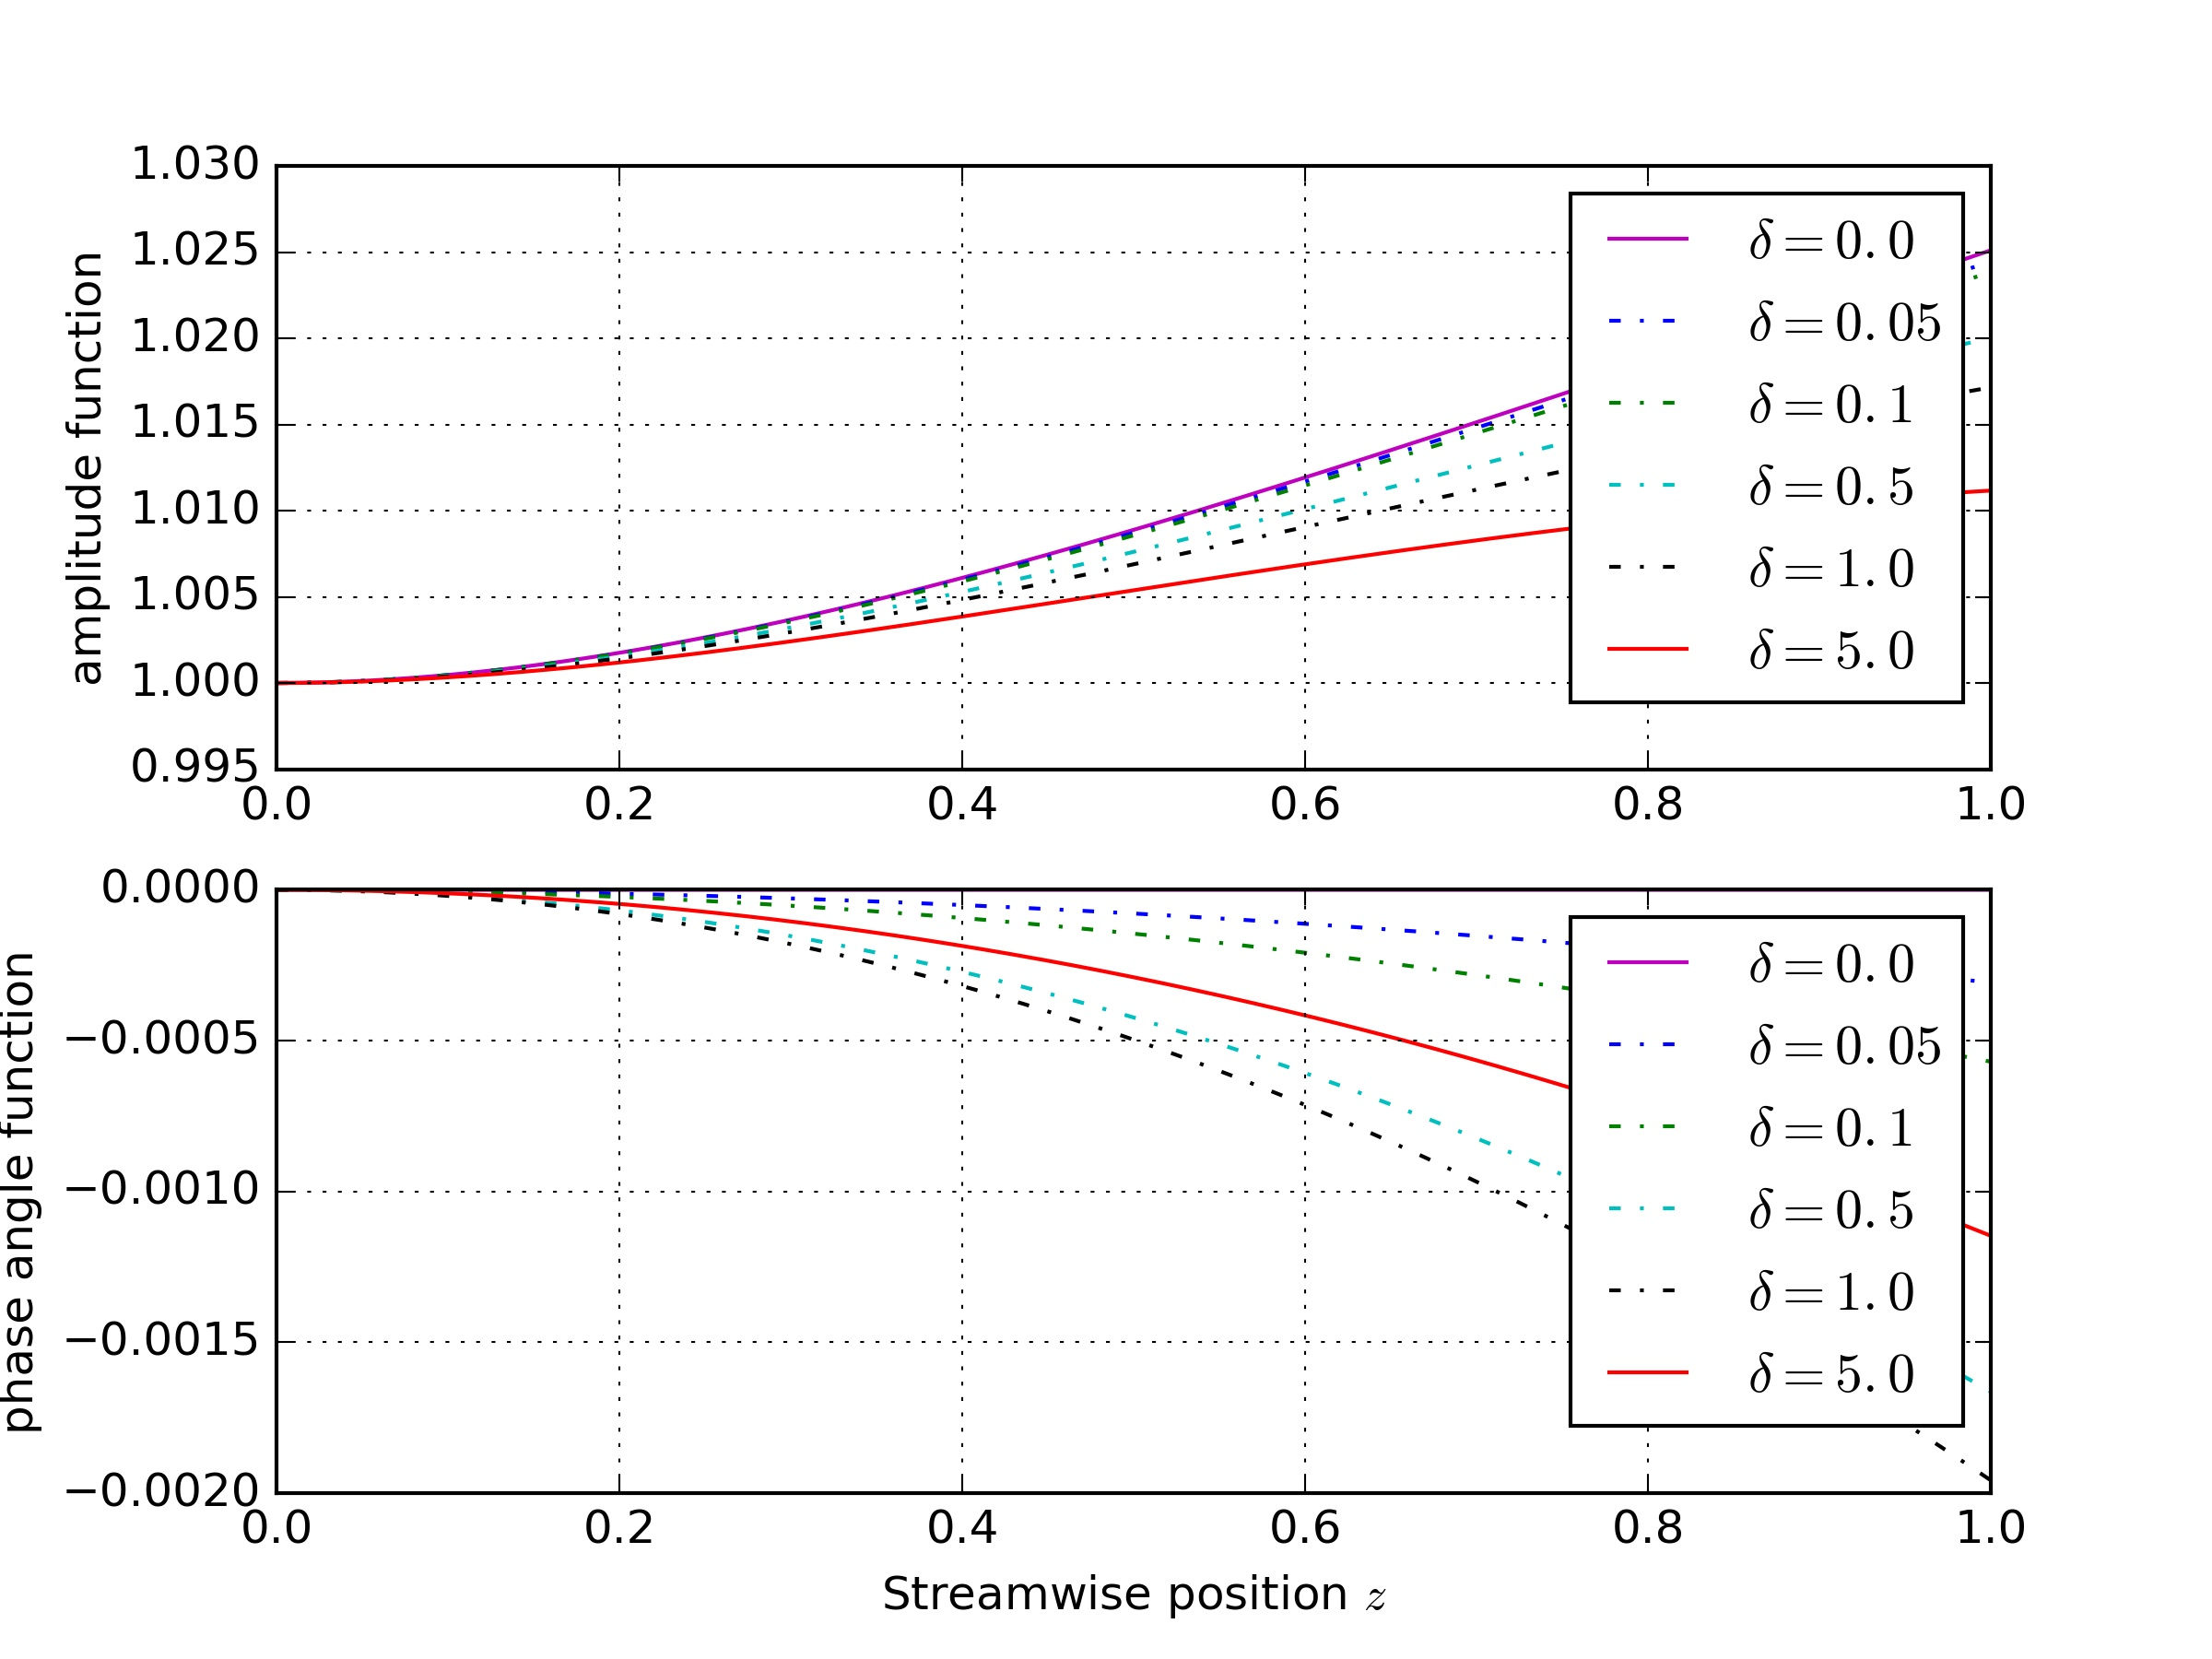
\includegraphics[width=\textwidth]{./img_eig_asy/fig_sol_analytic_disp_fun.jpg}
    \caption{Amplitude and phase of the displacement function $u(z)$}
    \label{fig:fig_sol_analytic_disp_fun}
\end{figure}

In the following, we can obtain the corresponding displacement function $u(z)$ in terms of its amplitude and phase in Figure~\ref{fig:fig_sol_analytic_disp_fun}. 


For a typical piezoelectric cantilever energy harvester in the literature \cite{erturk2008distributed,erturk2009experimentally}, this parameter $\delta$ is rather small



Using the following regular expansion:
\begin{equation}
    \left\{\begin{aligned}
        A_\epsilon &= A_0 + \epsilon A_1 + \epsilon^2 A_2 + \cdots, \\
        B_\epsilon &= B_0 + \epsilon B_1 + \epsilon^2 B_2 + \cdots, \\
        C_\epsilon &= C_0 + \epsilon C_1 + \epsilon^2 C_2 + \cdots, \\
        D_\epsilon &= D_0 + \epsilon D_1 + \epsilon^2 D_2 + \cdots, 
    \end{aligned}\right.
\end{equation}
we obtain the successive expansion problem:

\noindent
$O(\epsilon^0)$:
\begin{equation}
    \left\{\begin{aligned}
        A_0 + C_0 &= 1, \\
        B_0 + D_0 &= 0, \\
        - A_0 \cos{\sqrt{\sigma}} - B_0 \sin{\sqrt{\sigma}} + C_0 \cosh{\sqrt{\sigma}} + D_0 \sinh{\sqrt{\sigma}} &= 0, \\
        A_0 \sin{\sqrt{\sigma}} - B_0 \cos{\sqrt{\sigma}} + C_0 \sinh{\sqrt{\sigma}} + D_0 \cosh{\sqrt{\sigma}} &= 0.
    \end{aligned}\right.
\end{equation}
The solution is
\begin{equation}
    \left\{\begin{aligned}
        A_0 &= \frac{1 + \cos\sqrt{\sigma} \cosh\sqrt{\sigma} - \sin\sqrt{\sigma} \sinh\sqrt{\sigma} }{2 + 2 \cos\sqrt{\sigma} \cosh\sqrt{\sigma} } \\
        B_0 &= \frac{\cosh\sqrt{\sigma} \sin\sqrt{\sigma} + \cos\sqrt{\sigma} \sinh\sqrt{\sigma} }{2 + 2 \cos\sqrt{\sigma} \cosh\sqrt{\sigma} } \\
        C_0 &= \frac{1 + \cos\sqrt{\sigma} \cosh\sqrt{\sigma} + \sin\sqrt{\sigma} \sinh\sqrt{\sigma} }{2 + 2 \cos\sqrt{\sigma} \cosh\sqrt{\sigma} } \\
        D_0 &= -\frac{\cosh\sqrt{\sigma} \sin\sqrt{\sigma} + \cos\sqrt{\sigma} \sinh\sqrt{\sigma} }{2 + 2 \cos\sqrt{\sigma} \cosh\sqrt{\sigma} }
    \end{aligned}\right.
\end{equation}
Hence we have
\begin{equation}
    - A_0 \sin{\sqrt{\sigma}} + B_0 \cos{\sqrt{\sigma}} + C_0 \sinh{\sqrt{\sigma}} + D_0 \cosh{\sqrt{\sigma}} = \frac{\sinh\sqrt{\sigma }-\sin\sqrt{\sigma }}{\cos\sqrt{\sigma } \cosh\sqrt{\sigma }+1}
\end{equation}

\noindent
$O(\epsilon^1)$:
\begin{equation}
    \left\{\begin{aligned}
        A_1 + C_1 &= 0, \\
        B_1 + D_1 &= 0, \\
        \left( - A_1 \cos{\sqrt{\sigma}} - B_1 \sin{\sqrt{\sigma}} + C_1 \cosh{\sqrt{\sigma}} + D_1 \sinh{\sqrt{\sigma}} \right) &+ \\
        \frac{j \beta \sqrt{\sigma}}{ j\sigma \beta + 1 } \left( - A_0 \sin{\sqrt{\sigma}} + B_0 \cos{\sqrt{\sigma}} + C_0 \sinh{\sqrt{\sigma}} + D_0 \cosh{\sqrt{\sigma}} \right) &= 0, \\
        A_1 \sin{\sqrt{\sigma}} - B_1 \cos{\sqrt{\sigma}} + C_1 \sinh{\sqrt{\sigma}} + D_1 \cosh{\sqrt{\sigma}} &= 0.
    \end{aligned}\right.
\end{equation}
The solution is
\begin{equation}
    \left\{\begin{aligned}
        A_1 &= \frac{j \beta  \sqrt{\sigma }}{1+j \beta  \sigma } \left( \frac{\sinh\sqrt{\sigma }-\sin\sqrt{\sigma }}{\cos\sqrt{\sigma } \cosh\sqrt{\sigma }+1} \right) \left(\frac{\cos\sqrt{\sigma }+\cosh\sqrt{\sigma }}{2 \cos\sqrt{\sigma }\cosh\sqrt{\sigma }+2} \right) \\
        B_1 &= \frac{j \beta  \sqrt{\sigma }}{1+j \beta  \sigma } \left( \frac{\sinh\sqrt{\sigma }-\sin\sqrt{\sigma }}{\cos\sqrt{\sigma } \cosh\sqrt{\sigma }+1} \right) \left( \frac{-\sinh\sqrt{\sigma }+\sin\sqrt{\sigma }}{2 \cos\sqrt{\sigma }\cosh\sqrt{\sigma }+2} \right)\\
        C_1 &= \frac{j \beta  \sqrt{\sigma }}{1+j \beta  \sigma } \left( \frac{\sinh\sqrt{\sigma }-\sin\sqrt{\sigma }}{\cos\sqrt{\sigma } \cosh\sqrt{\sigma }+1} \right) \left( -\frac{\cos\sqrt{\sigma }+\cosh\sqrt{\sigma }}{2 \cos\sqrt{\sigma } \cosh\sqrt{\sigma }+2} \right)\\
        D_1 &= \frac{j \beta  \sqrt{\sigma }}{1+j \beta  \sigma } \left( \frac{\sinh\sqrt{\sigma }-\sin\sqrt{\sigma }}{\cos\sqrt{\sigma } \cosh\sqrt{\sigma }+1} \right) \left( \frac{-\sin\sqrt{\sigma }+\sinh\sqrt{\sigma }}{2 \cos\sqrt{\sigma }\cosh\sqrt{\sigma }+2} \right)
    \end{aligned}\right.
\end{equation}
Then we have
\begin{equation}
    \begin{aligned}
        - A_1 \sin{\sqrt{\sigma}} + B_1 \cos{\sqrt{\sigma}} + C_1 \sinh{\sqrt{\sigma}} + D_1 \cosh{\sqrt{\sigma}} \\
        = \frac{j \beta  \sqrt{\sigma }}{1+j \beta  \sigma } \left(\frac{\sin\sqrt{\sigma } -\sinh\sqrt{\sigma }}{\cos\sqrt{\sigma } \cosh\sqrt{\sigma }+1} \right)  \left( \frac{\cos\sqrt{\sigma } \sinh\sqrt{\sigma }+\sin\sqrt{\sigma } \cosh\sqrt{\sigma }}{\cos\sqrt{\sigma } \cosh\sqrt{\sigma }+1} \right)
    \end{aligned}
\end{equation}

\noindent
$O(\epsilon^2)$:
\begin{equation}
    \left\{\begin{aligned}
        A_2 + C_2 &= 0, \\
        B_2 + D_2 &= 0, \\
        \left( - A_2 \cos{\sqrt{\sigma}} - B_2 \sin{\sqrt{\sigma}} + C_2 \cosh{\sqrt{\sigma}} + D_2 \sinh{\sqrt{\sigma}} \right) &+ \\
        \frac{j \beta \sqrt{\sigma}}{ j\sigma \beta + 1 } \left( - A_1 \sin{\sqrt{\sigma}} + B_1 \cos{\sqrt{\sigma}} + C_1 \sinh{\sqrt{\sigma}} + D_1 \cosh{\sqrt{\sigma}} \right) &= 0, \\
        A_2 \sin{\sqrt{\sigma}} - B_2 \cos{\sqrt{\sigma}} + C_2 \sinh{\sqrt{\sigma}} + D_2 \cosh{\sqrt{\sigma}} &= 0.
    \end{aligned}\right.
\end{equation}
The solution is
\scriptsize
\begin{equation}
    \left\{\begin{aligned}
        A_2 &= \left( \frac{j \beta \sqrt{\sigma }}{1+j \beta \sigma } \right)^2 \left(\frac{ \sinh\sqrt{\sigma } - \sin\sqrt{\sigma }}{\cos\sqrt{\sigma } \cosh\sqrt{\sigma }+1} \right) \left( \frac{\cos\sqrt{\sigma } \sinh\sqrt{\sigma }+\sin\sqrt{\sigma } \cosh\sqrt{\sigma }}{\cos\sqrt{\sigma } \cosh\sqrt{\sigma }+1} \right) \left(\frac{\cos\sqrt{\sigma }+\cosh\sqrt{\sigma }}{2 \cos\sqrt{\sigma }\cosh\sqrt{\sigma }+2} \right) \\
        B_2 &= \left( \frac{j \beta \sqrt{\sigma }}{1+j \beta \sigma } \right)^2 \left(\frac{\sinh\sqrt{\sigma } - \sin\sqrt{\sigma }}{\cos\sqrt{\sigma } \cosh\sqrt{\sigma }+1} \right) \left( \frac{\cos\sqrt{\sigma } \sinh\sqrt{\sigma }+\sin\sqrt{\sigma } \cosh\sqrt{\sigma }}{\cos\sqrt{\sigma } \cosh\sqrt{\sigma }+1} \right) \left( \frac{-\sinh\sqrt{\sigma }+\sin\sqrt{\sigma }}{2 \cos\sqrt{\sigma }\cosh\sqrt{\sigma }+2} \right)\\
        C_2 &= \left( \frac{j \beta \sqrt{\sigma }}{1+j \beta \sigma } \right)^2 \left(\frac{\sinh\sqrt{\sigma } - \sin\sqrt{\sigma }}{\cos\sqrt{\sigma } \cosh\sqrt{\sigma }+1} \right) \left( \frac{\cos\sqrt{\sigma } \sinh\sqrt{\sigma }+\sin\sqrt{\sigma } \cosh\sqrt{\sigma }}{\cos\sqrt{\sigma } \cosh\sqrt{\sigma }+1} \right) \left( -\frac{\cos\sqrt{\sigma }+\cosh\sqrt{\sigma }}{2 \cos\sqrt{\sigma } \cosh\sqrt{\sigma }+2} \right)\\
        D_2 &= \left( \frac{j \beta \sqrt{\sigma }}{1+j \beta \sigma } \right)^2 \left(\frac{\sinh\sqrt{\sigma } - \sin\sqrt{\sigma }}{\cos\sqrt{\sigma } \cosh\sqrt{\sigma }+1} \right) \left( \frac{\cos\sqrt{\sigma } \sinh\sqrt{\sigma }+\sin\sqrt{\sigma } \cosh\sqrt{\sigma }}{\cos\sqrt{\sigma } \cosh\sqrt{\sigma }+1} \right) \left( \frac{-\sin\sqrt{\sigma }+\sinh\sqrt{\sigma }}{2 \cos\sqrt{\sigma }\cosh\sqrt{\sigma }+2} \right)
    \end{aligned}\right.
\end{equation}
\normalsize

To get higher order expansions, we can use the following iteration method:

\noindent
$O(\epsilon^{k+1})\ (k\geq 1)$:
\begin{equation}
    \left\{\begin{aligned}
        A_{k+1} + C_{k+1} &= 0, \\
        B_{k+1} + D_{k+1} &= 0, \\
        \left( - A_{k+1} \cos{\sqrt{\sigma}} - B_{k+1} \sin{\sqrt{\sigma}} + C_{k+1} \cosh{\sqrt{\sigma}} + D_{k+1} \sinh{\sqrt{\sigma}} \right) &+ \\
        \frac{j \beta \sqrt{\sigma}}{ j\sigma \beta + 1 } \left( - A_{k} \sin{\sqrt{\sigma}} + B_{k} \cos{\sqrt{\sigma}} + C_{k} \sinh{\sqrt{\sigma}} + D_{k} \cosh{\sqrt{\sigma}} \right) &= 0, \\
        A_{k+1} \sin{\sqrt{\sigma}} - B_{k+1} \cos{\sqrt{\sigma}} + C_{k+1} \sinh{\sqrt{\sigma}} + D_{k+1} \cosh{\sqrt{\sigma}} &= 0.
    \end{aligned}\right.
\end{equation}
The solution is
\begin{equation}
    \left\{\begin{aligned}
        A_{k+1} &= \left( \frac{j \beta \sqrt{\sigma }}{1+j \beta \sigma } \right) \left(\frac{\cos\sqrt{\sigma }+\cosh\sqrt{\sigma }}{2 \cos\sqrt{\sigma }\cosh\sqrt{\sigma }+2} \right) \left( Q_k \right) \\
        B_{k+1} &= \left( \frac{j \beta \sqrt{\sigma }}{1+j \beta \sigma } \right) \left( \frac{-\sinh\sqrt{\sigma }+\sin\sqrt{\sigma }}{2 \cos\sqrt{\sigma }\cosh\sqrt{\sigma }+2} \right) \left( Q_k \right) \\
        C_{k+1} &= \left( \frac{j \beta \sqrt{\sigma }}{1+j \beta \sigma } \right) \left( -\frac{\cos\sqrt{\sigma }+\cosh\sqrt{\sigma }}{2 \cos\sqrt{\sigma } \cosh\sqrt{\sigma }+2} \right) \left( Q_k \right) \\
        D_{k+1} &= \left( \frac{j \beta \sqrt{\sigma }}{1+j \beta \sigma } \right) \left( \frac{-\sin\sqrt{\sigma }+\sinh\sqrt{\sigma }}{2 \cos\sqrt{\sigma }\cosh\sqrt{\sigma }+2} \right) \left( Q_k \right) 
    \end{aligned}\right.
\end{equation}
where for $k \geq 2$
\begin{equation}
    Q_k = - A_{k} \sin{\sqrt{\sigma}} + B_{k} \cos{\sqrt{\sigma}} + C_{k} \sinh{\sqrt{\sigma}} + D_{k} \cosh{\sqrt{\sigma}},
\end{equation}
and for $k \geq 0$
\begin{equation}
    \begin{aligned}
        Q_{k+1} &= - A_{k+1} \sin{\sqrt{\sigma}} + B_{k+1} \cos{\sqrt{\sigma}} + C_{k+1} \sinh{\sqrt{\sigma}} + D_{k+1} \cosh{\sqrt{\sigma}} \\
        &= - \left( \frac{ \sin\sqrt{\sigma} \cosh\sqrt{\sigma} + \cos\sqrt{\sigma} \sinh\sqrt{\sigma} }{ \cos\sqrt{\sigma }\cosh\sqrt{\sigma }+1 } \right) \left( \frac{j \beta \sqrt{\sigma }}{1+j \beta \sigma } \right) Q_k,
    \end{aligned}
\end{equation}
and
\begin{equation}
    \begin{aligned}
        Q_{1} &= - A_1 \sin{\sqrt{\sigma}} + B_1 \cos{\sqrt{\sigma}} + C_1 \sinh{\sqrt{\sigma}} + D_1 \cosh{\sqrt{\sigma}} \\
        &= \frac{j \beta  \sqrt{\sigma }}{1+j \beta  \sigma } \left(\frac{\sin\sqrt{\sigma } -\sinh\sqrt{\sigma }}{\cos\sqrt{\sigma } \cosh\sqrt{\sigma }+1} \right)  \left( \frac{\cos\sqrt{\sigma } \sinh\sqrt{\sigma }+\sin\sqrt{\sigma } \cosh\sqrt{\sigma }}{\cos\sqrt{\sigma } \cosh\sqrt{\sigma }+1} \right)
    \end{aligned}
\end{equation}
\begin{equation}
    Q_0 = \frac{\sinh\sqrt{\sigma }-\sin\sqrt{\sigma }}{\cos\sqrt{\sigma } \cosh\sqrt{\sigma }+1}
\end{equation}

Hence it is shown that for $k \geq 0$
\begin{equation}
    \begin{aligned}
        Q_{k} &= - \left( \frac{ \sin\sqrt{\sigma} \cosh\sqrt{\sigma} + \cos\sqrt{\sigma} \sinh\sqrt{\sigma} }{ \cos\sqrt{\sigma }\cosh\sqrt{\sigma }+1 } \right) \left( \frac{j \beta \sqrt{\sigma }}{1+j \beta \sigma } \right) Q_k \\
        &= \left[- \left( \frac{j \beta \sqrt{\sigma }}{1+j \beta \sigma } \right) \left( \frac{ \sin\sqrt{\sigma} \cosh\sqrt{\sigma} + \cos\sqrt{\sigma} \sinh\sqrt{\sigma} }{ \cos\sqrt{\sigma }\cosh\sqrt{\sigma }+1 } \right)  \right]^k \left( \frac{\sinh\sqrt{\sigma }-\sin\sqrt{\sigma }}{\cos\sqrt{\sigma } \cosh\sqrt{\sigma }+1} \right)
    \end{aligned}
\end{equation}

As a result, we obtain that for $k \geq 0$
\scriptsize
\begin{equation}
    \left\{\begin{aligned}
        A_{k+1} &= \left( \frac{j \beta \sqrt{\sigma }}{1+j \beta \sigma } \right)^{k+1} \left( \frac{ -\sin\sqrt{\sigma} \cosh\sqrt{\sigma} - \cos\sqrt{\sigma} \sinh\sqrt{\sigma} }{ \cos\sqrt{\sigma }\cosh\sqrt{\sigma }+1 } \right)^k \left( \frac{\sinh\sqrt{\sigma }-\sin\sqrt{\sigma }}{\cos\sqrt{\sigma } \cosh\sqrt{\sigma }+1} \right) \left(\frac{\cos\sqrt{\sigma }+\cosh\sqrt{\sigma }}{2 \cos\sqrt{\sigma }\cosh\sqrt{\sigma }+2} \right) \\
        B_{k+1} &= \left( \frac{j \beta \sqrt{\sigma }}{1+j \beta \sigma } \right)^{k+1}  \left( \frac{ -\sin\sqrt{\sigma} \cosh\sqrt{\sigma} - \cos\sqrt{\sigma} \sinh\sqrt{\sigma} }{ \cos\sqrt{\sigma }\cosh\sqrt{\sigma }+1 } \right)^k \left( \frac{\sinh\sqrt{\sigma }-\sin\sqrt{\sigma }}{\cos\sqrt{\sigma } \cosh\sqrt{\sigma }+1} \right) \left( \frac{-\sinh\sqrt{\sigma }+\sin\sqrt{\sigma }}{2 \cos\sqrt{\sigma }\cosh\sqrt{\sigma }+2} \right) \\
        C_{k+1} &= \left( \frac{j \beta \sqrt{\sigma }}{1+j \beta \sigma } \right)^{k+1}  \left( \frac{ -\sin\sqrt{\sigma} \cosh\sqrt{\sigma} - \cos\sqrt{\sigma} \sinh\sqrt{\sigma} }{ \cos\sqrt{\sigma }\cosh\sqrt{\sigma }+1 } \right)^k \left( \frac{\sinh\sqrt{\sigma }-\sin\sqrt{\sigma }}{\cos\sqrt{\sigma } \cosh\sqrt{\sigma }+1} \right) \left( \frac{-\cos\sqrt{\sigma }-\cosh\sqrt{\sigma }}{2 \cos\sqrt{\sigma } \cosh\sqrt{\sigma }+2} \right) \\
        D_{k+1} &= \left( \frac{j \beta \sqrt{\sigma }}{1+j \beta \sigma } \right)^{k+1} \left( \frac{ -\sin\sqrt{\sigma} \cosh\sqrt{\sigma} - \cos\sqrt{\sigma} \sinh\sqrt{\sigma} }{ \cos\sqrt{\sigma }\cosh\sqrt{\sigma }+1 } \right)^k \left( \frac{\sinh\sqrt{\sigma }-\sin\sqrt{\sigma }}{\cos\sqrt{\sigma } \cosh\sqrt{\sigma }+1} \right) \left( \frac{-\sin\sqrt{\sigma }+\sinh\sqrt{\sigma }}{2 \cos\sqrt{\sigma }\cosh\sqrt{\sigma }+2} \right)
    \end{aligned}\right.
\end{equation}
\normalsize























































\section*{Reference}

\bibliography{analysis_eig_asy.bib}
\bibliographystyle{vancouver}

\end{document}